\section{Architectural Choices}
\label{arch}

\subsection{Pure Inception blocks}

Our older Inception models used to be trained in a partitioned manner,
where each replica was partitioned into a multiple sub-networks in order to be able to
fit the whole model in memory. However, the Inception architecture is highly
tunable, meaning that there are a lot of possible changes to the number of filters
in the various layers that do not affect the quality of the fully trained
network. In order to optimize the training speed, we used to tune the layer sizes
carefully in order to balance the computation between the various model
sub-networks.
In contrast, with the introduction of TensorFlow our most recent models
can be trained without partitioning the replicas. This is enabled in part by recent
optimizations of memory used by backpropagation, achieved by carefully considering
what tensors are needed for gradient computation and structuring the computation
to reduce the number of such tensors. Historically, we have been
relatively conservative about changing the architectural choices and restricted
our experiments to varying isolated network components while keeping the
rest of the network stable. Not simplifying earlier choices
resulted in networks that looked more complicated that they needed to be.
In our newer experiments, for Inception-v4 we decided to shed this unnecessary
baggage and made uniform choices for the Inception blocks for each grid size.
Plase refer to Figure~\ref{fig:inceptionv4} for the large scale
structure of the Inception-v4 network and Figures~\ref{fig:inceptionv4stem},
\ref{fig:wide35x35module}, \ref{fig:wide17x17module}, \ref{fig:wide8x8module},
\ref{fig:reductionto17} and \ref{fig:reductionto8} for the detailed structure
of its components. All the convolutions not marked with ``V'' in the figures
are same-padded meaning that their output grid matches the size of their input.
Convolutions marked with ``V'' are valid padded, meaning that input patch of
each unit is fully contained in the previous layer and the grid size of the
output activation map is reduced accordingly.

\subsection{Residual Inception Blocks}
For the residual versions of the Inception networks, we use cheaper Inception
blocks than the original Inception. Each Inception block is followed by
filter-expansion layer ($1\times 1$ convolution without activation) which is
used for scaling up the dimensionality of the filter bank before the addition
to match the depth of the input. This is needed to compensate for the dimensionality
reduction induced by the Inception block.

We tried several versions of the residual version of Inception. Only two
of them are detailed here. The first one ``Inception-ResNet-v1''
roughly the computational cost of Inception-v3, while ``Inception-ResNet-v2''
matches the raw cost of the newly introduced Inception-v4 network. See
Figure~\ref{fig:resnetsmallschema} for the large scale structure of both
varianets. (However, the step time of Inception-v4 proved to be significantly
slower in practice, probably due to the larger number of layers.)

Another small technical difference between our residual and non-residual
Inception variants is that in the case of Inception-ResNet,
we used batch-normalization only on top of the traditional layers, but not
on top of the summations. It is reasonable to expect that a thorough use
of batch-normalization should be advantageous, but we wanted to keep
each model replica trainable on a single GPU. It turned out that the
memory footprint of layers with large activation size was consuming
disproportionate amount of GPU-memory. By omitting the batch-normalization
on top of those layers, we were able to increase the overall number of
Inception blocks substantially. We hope that with better utilization of
computing resources, making this trade-off will become unecessary.

\begin{figure}
\centering
\includegraphics[width=0.7\linewidth]{inceptionv4stem}
\caption{The schema for stem of the pure Inception-v4 and
  Inception-ResNet-v2 networks. This is the input part of those
networks. Cf. Figures~\ref{fig:inceptionv4} and~\ref{fig:resnetsmallschema} }
\label{fig:inceptionv4stem}
\end{figure}
\begin{figure}
\centering
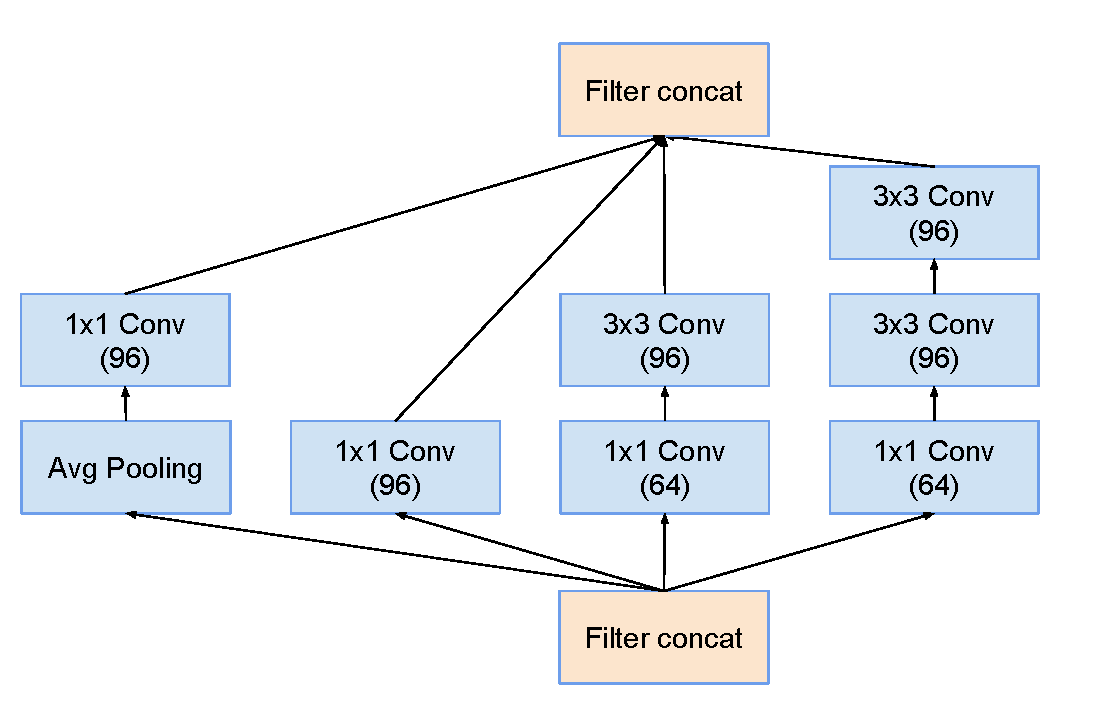
\includegraphics[width=\linewidth]{wide35x35module}
\caption{The schema for $35\times 35$ grid modules of the pure Inception-v4
 network. This is the Inception-A block of Figure~\ref{fig:inceptionv4}. }
\label{fig:wide35x35module}
\end{figure}
\begin{figure}
\centering
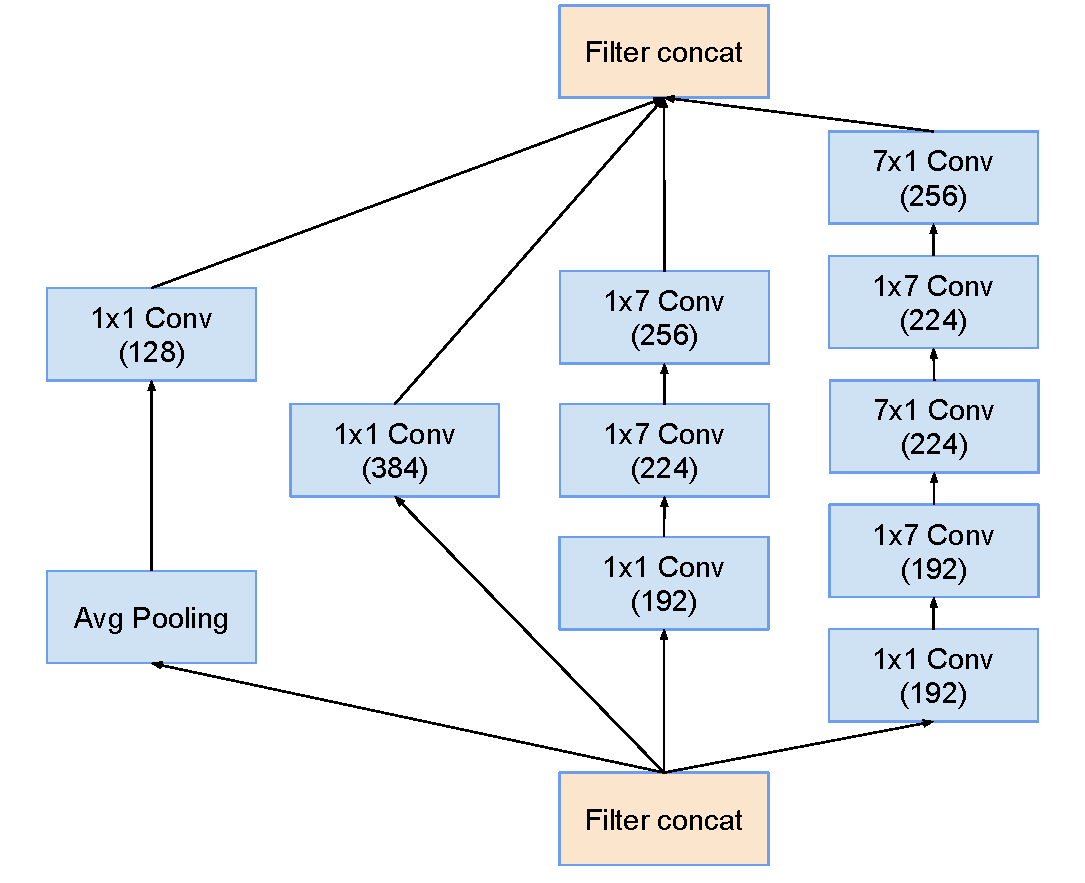
\includegraphics[width=\linewidth]{wide17x17module}
\caption{The schema for $17\times 17$ grid modules of the pure Inception-v4
 network. This is the Inception-B block of Figure~\ref{fig:inceptionv4}.}
\label{fig:wide17x17module}
\end{figure}
\begin{figure}
\centering
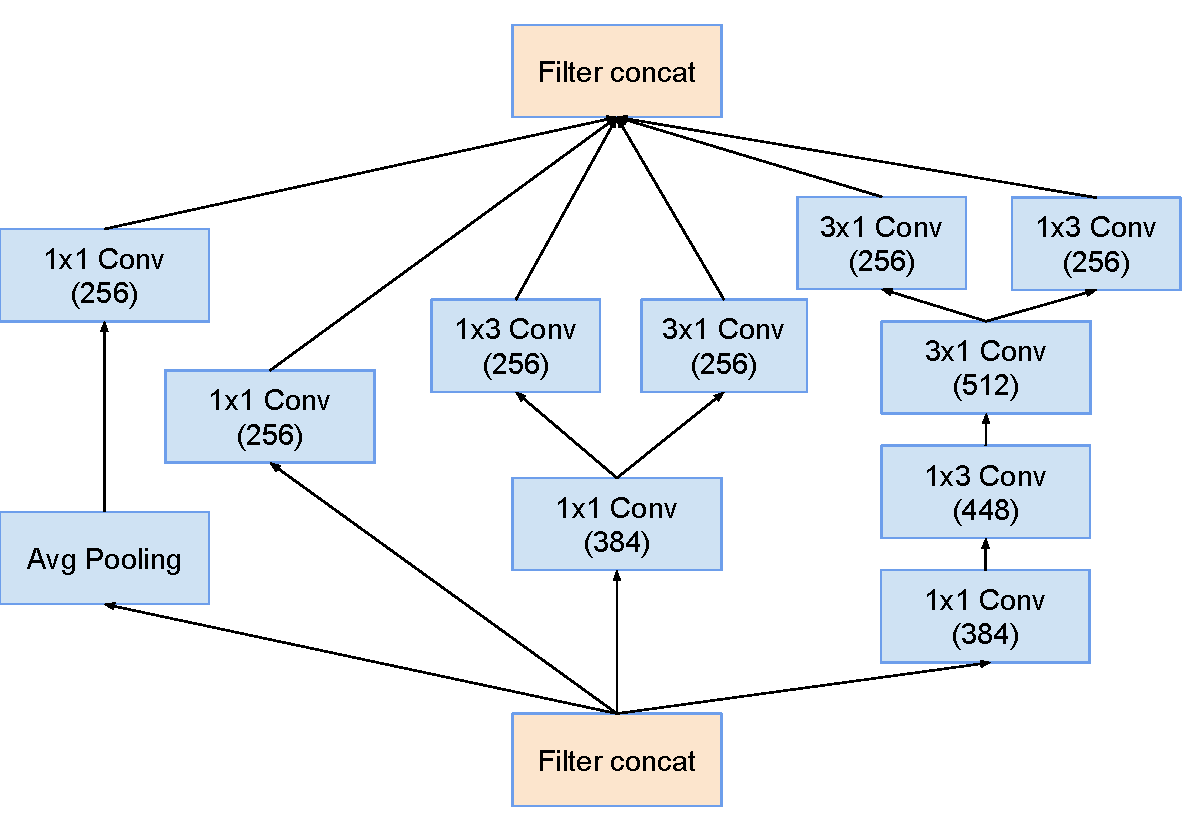
\includegraphics[width=\linewidth]{wide8x8module}
\caption{The schema for $8\times 8$ grid modules of the pure Inception-v4
 network. This is the Inception-C block of Figure~\ref{fig:inceptionv4}.}
\label{fig:wide8x8module}
\end{figure}
\begin{figure}
\centering
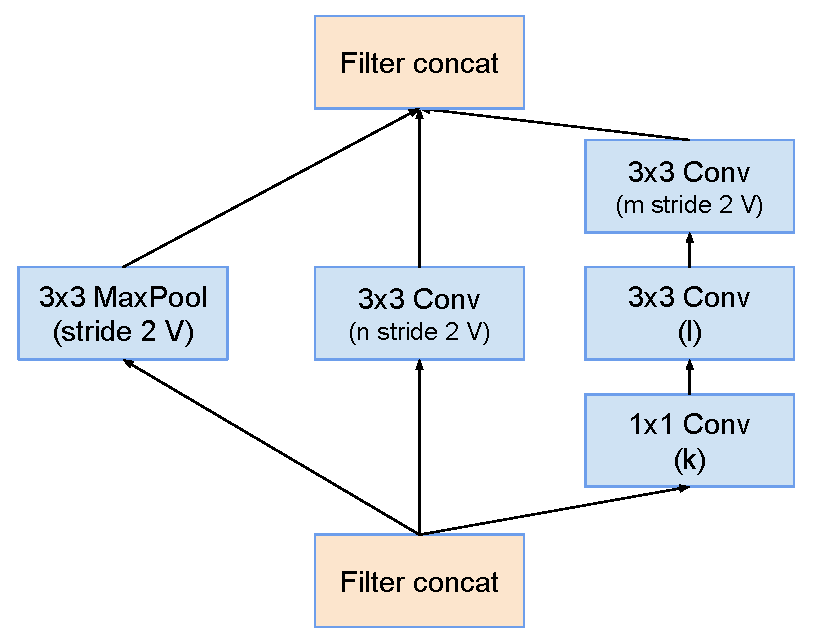
\includegraphics[width=\linewidth]{reductionto17}
\caption{The schema for $35\times 35$ to $17\times 17$ reduction module.
  Different variants of this blocks (with various number of filters) are
  used in Figure~\ref{fig:inceptionv4}, and \ref{fig:resnetsmallschema}
  in each of the new Inception(-v4, -ResNet-v1, -ResNet-v2) variants
  presented in this paper. The $k$, $l$, $m$, $n$ numbers represent
  filter bank sizes which can be looked up in Table~\ref{reductionto17params}.
}
\label{fig:reductionto17}
\end{figure}
\begin{figure}
\centering
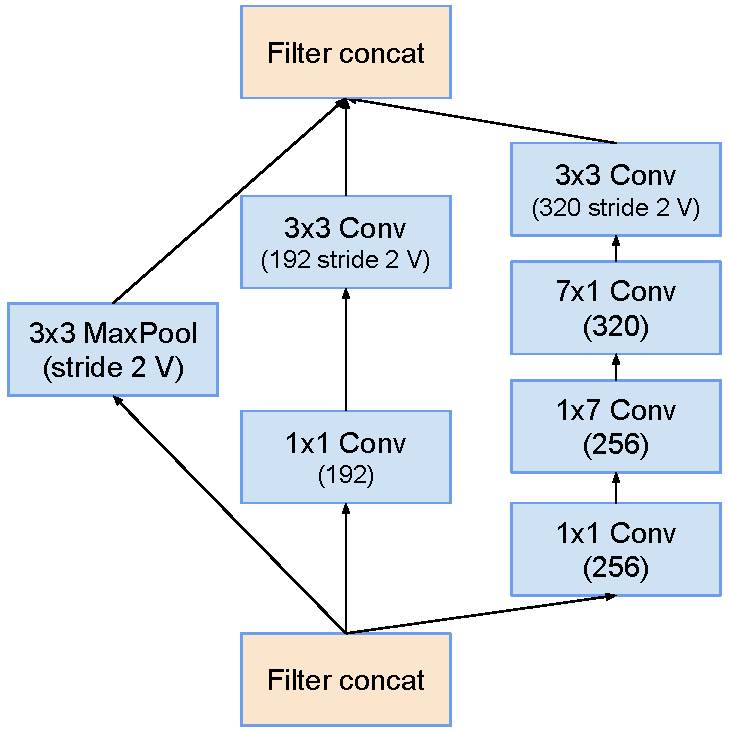
\includegraphics[width=\linewidth]{reductionto8}
\caption{The schema for $17\times 17$ to $8\times 8$ grid-reduction module.
  This is the reduction module used by the pure Inception-v4 network in
  Figure~\ref{fig:inceptionv4}.
}
\label{fig:reductionto8}
\end{figure}
\begin{figure}
\centering
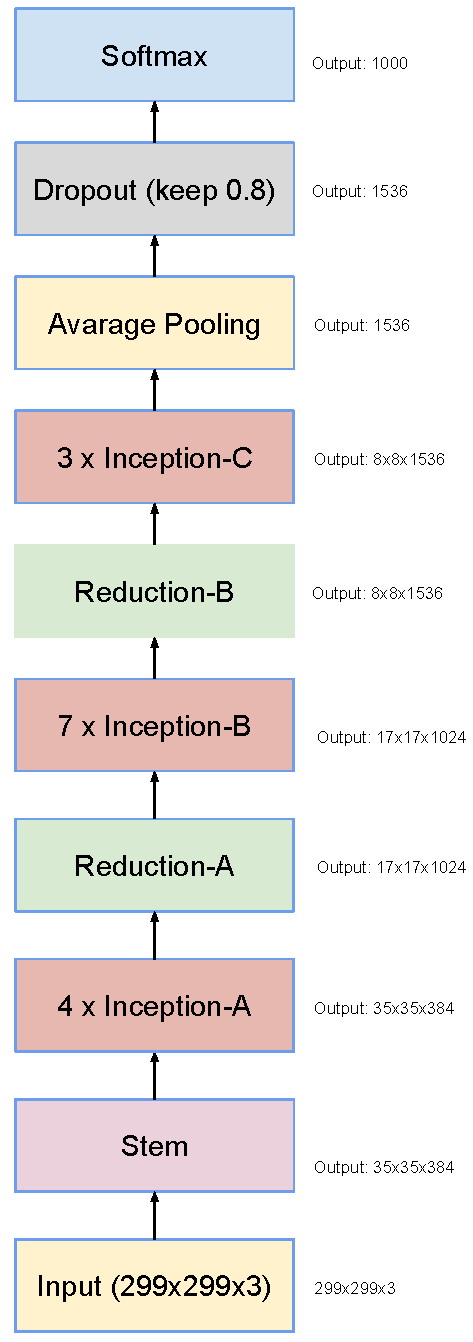
\includegraphics[width=0.5\linewidth]{inceptionv4}
\caption{The overall schema of the Inception-v4 network. For the
  detailed modules, please refer to Figures~\ref{fig:inceptionv4stem},
  \ref{fig:wide35x35module}, \ref{fig:wide17x17module}, \ref{fig:wide8x8module},
  \ref{fig:reductionto17} and \ref{fig:reductionto8} for the detailed structure
  of the various components.
}
\label{fig:inceptionv4}
\end{figure}
\begin{figure}
\centering
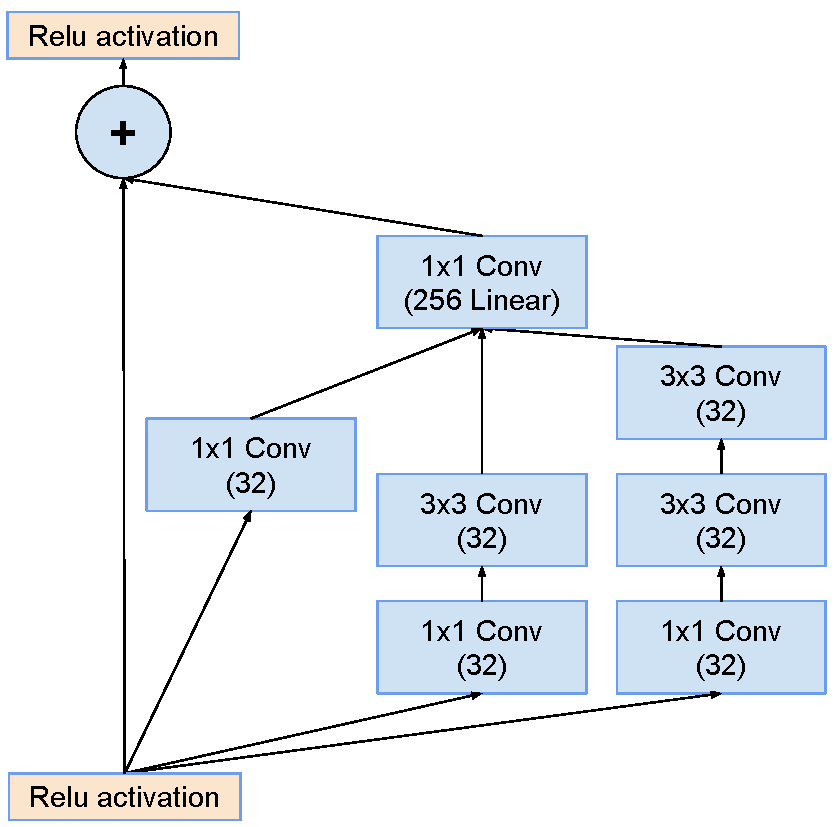
\includegraphics[width=\linewidth]{resnetsmall35x35}
\caption{The schema for $35\times 35$ grid (Inception-ResNet-A) module of Inception-ResNet-v1
 network.}
\label{fig:resnetsmall35x35module}
\end{figure}
\begin{figure}
\centering
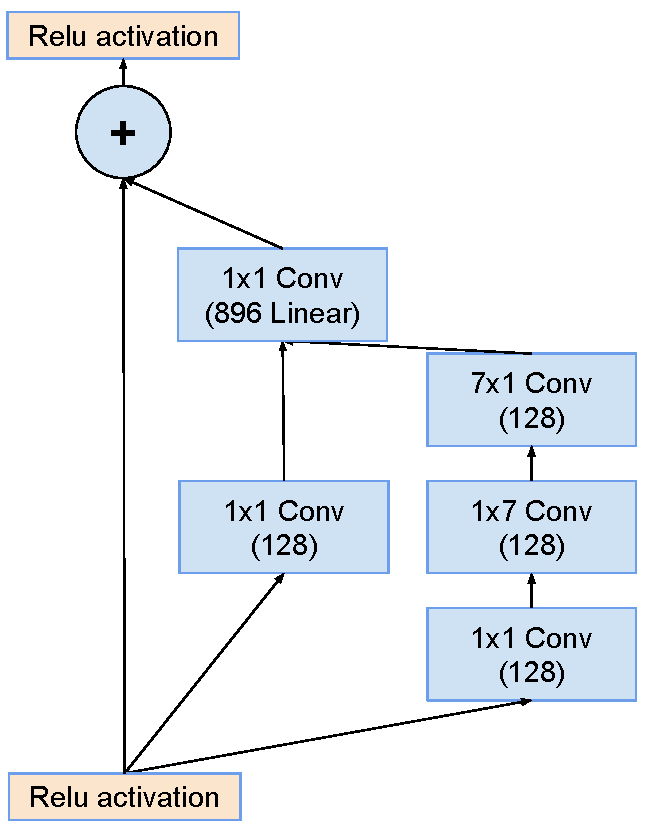
\includegraphics[width=\linewidth]{resnetsmall17x17}
\caption{The schema for $17\times 17$ grid (Inception-ResNet-B)  module of Inception-ResNet-v1
 network.}
\label{fig:resnetsmall17x17module}
\end{figure}
\begin{figure}
\centering
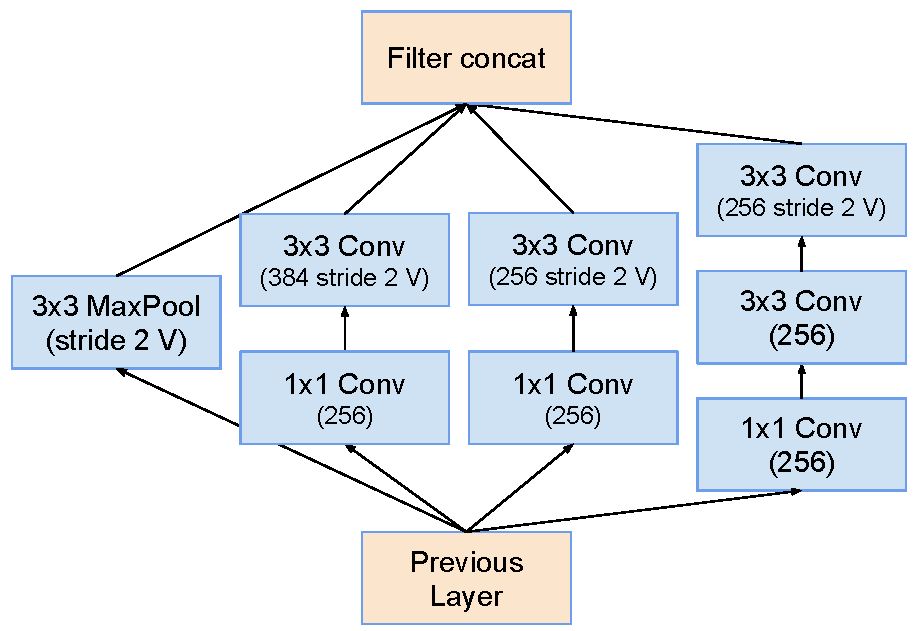
\includegraphics[width=\linewidth]{reductionto8resnet}
\caption{``Reduction-B'' $17\times 17$ to $8\times 8$ grid-reduction module.
  This module used by the smaller Inception-ResNet-v1 network
  in Figure~\ref{fig:resnetsmallschema}.
}
\label{fig:reductionto8resnet}
\end{figure}
\begin{figure}
\centering
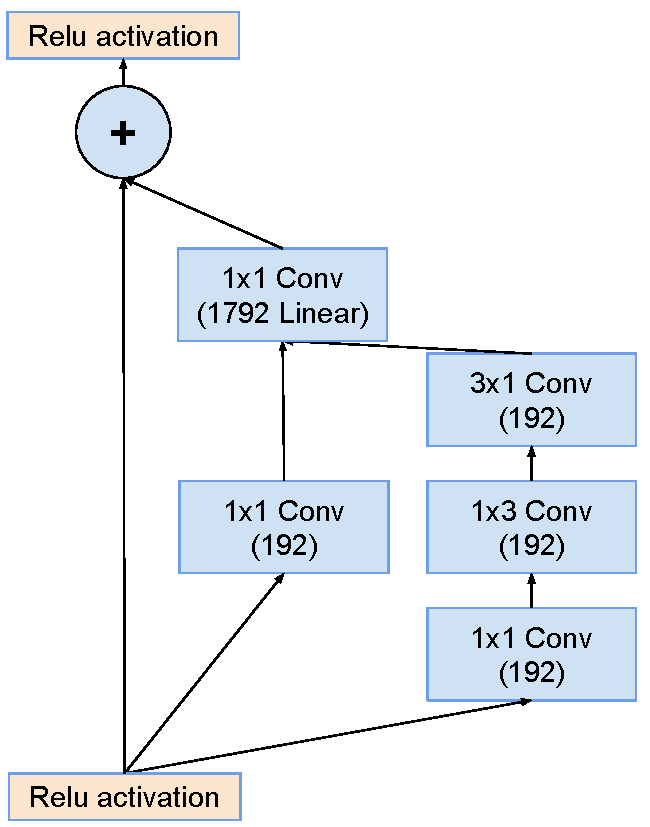
\includegraphics[width=\linewidth]{resnetsmall8x8}
\caption{The schema for $8\times 8$ grid (Inception-ResNet-C) module of Inception-ResNet-v1
 network.}
\label{fig:resnetsmall8x8module}
\end{figure}
\begin{figure}
\centering
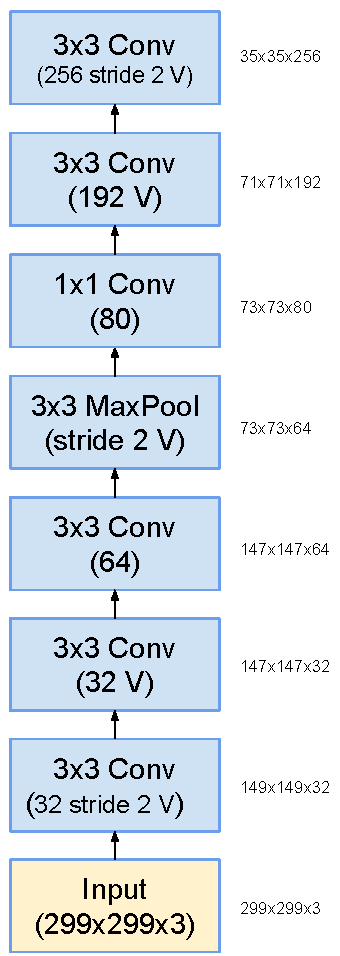
\includegraphics[width=0.5\linewidth]{ResnetSmallStem}
\caption{The stem of the Inception-ResNet-v1 network.}
\label{fig:resnetsmallstem}
\end{figure}
\begin{figure}
\centering
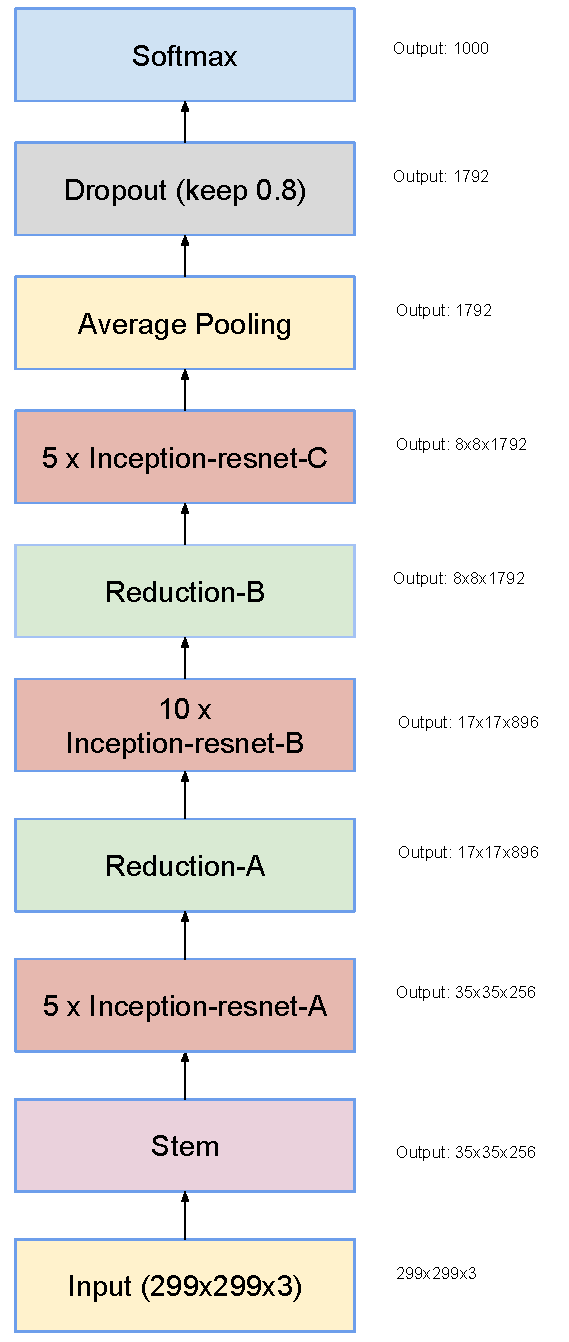
\includegraphics[width=0.5\linewidth]{inceptionresnetsmallschema}
\caption{Schema for Inception-ResNet-v1 and Inception-ResNet-v2 networks.
  This schema applies to both networks but the underlying components differ.
  Inception-ResNet-v1 uses the blocks as described in Figures~\ref{fig:resnetsmallstem},
  \ref{fig:resnetsmall35x35module}, \ref{fig:reductionto17}, \ref{fig:resnetsmall17x17module},
  \ref{fig:reductionto8resnet} and \ref{fig:resnetsmall8x8module}.
  Inception-ResNet-v2 uses the blocks as described in Figures~\ref{fig:inceptionv4stem},
  \ref{fig:resnetwide35x35module}, \ref{fig:reductionto17},\ref{fig:resnetwide17x17module},
  \ref{fig:reductionto8resnetwide} and \ref{fig:resnetwide8x8module}.
  The output sizes in the diagram refer to the activation vector tensor shapes of
  Inception-ResNet-v1.
}
\label{fig:resnetsmallschema}
\end{figure}
\clearpage
\begin{figure}
\centering
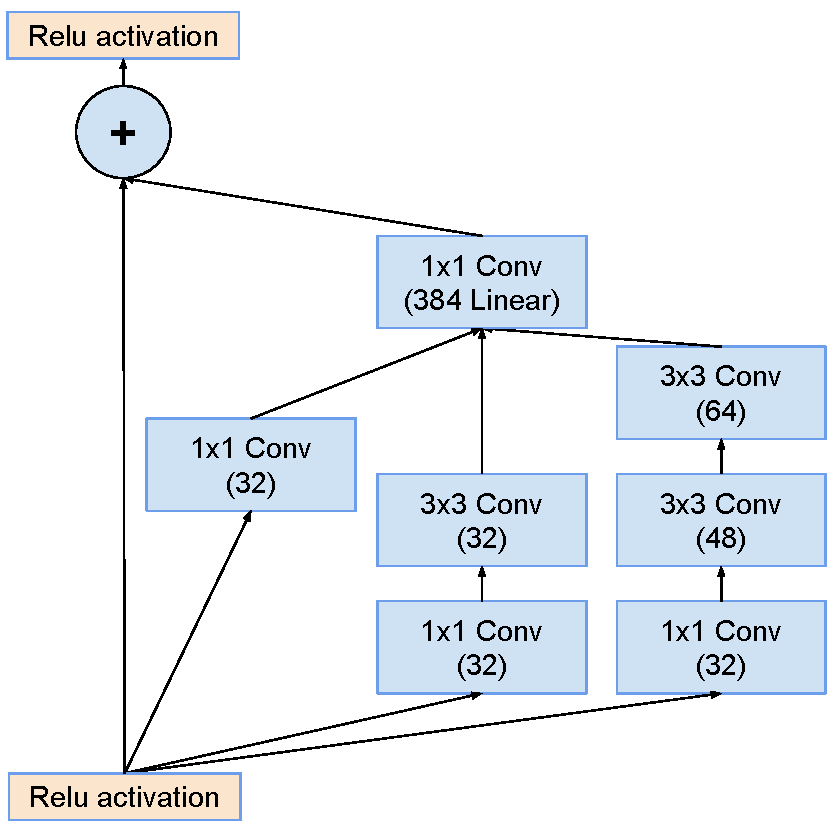
\includegraphics[width=\linewidth]{resnetwide35x35}\caption{The schema for
  $35\times 35$ grid (Inception-ResNet-A) module of the Inception-ResNet-v2 network.}
\label{fig:resnetwide35x35module}
\end{figure}
\begin{figure}
\centering
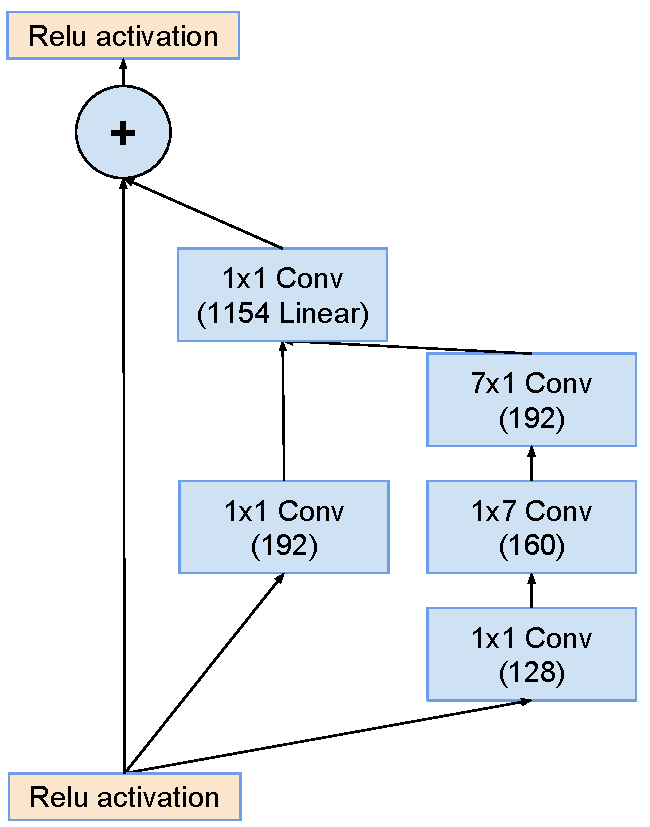
\includegraphics[width=\linewidth]{resnetwide17x17}
\caption{The schema for $17\times 17$ grid (Inception-ResNet-B) module of the
  Inception-ResNet-v2  network.}
\label{fig:resnetwide17x17module}
\end{figure}
\begin{figure}
\centering
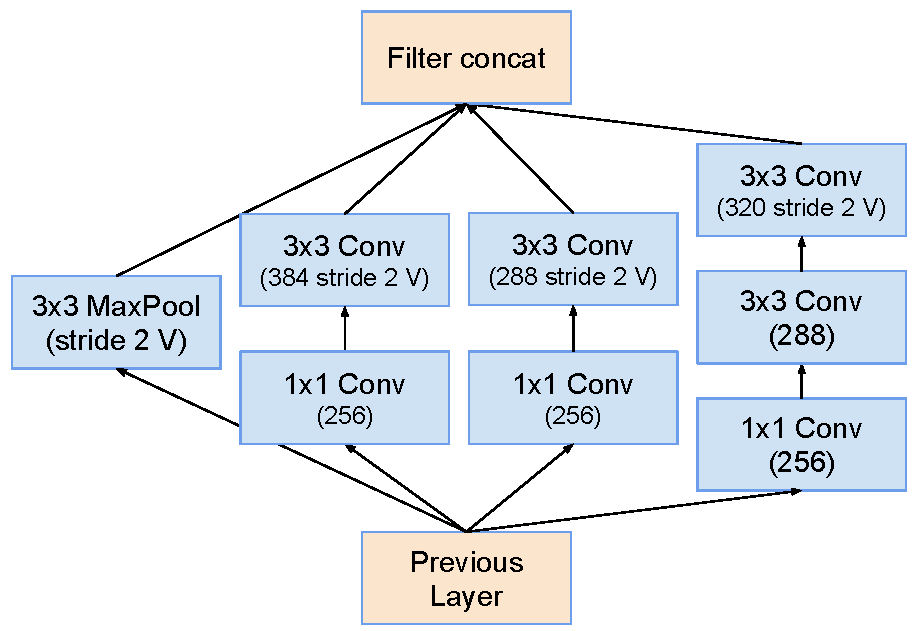
\includegraphics[width=\linewidth]{reductionto8resnetwide}
\caption{The schema for $17\times 17$ to $8\times 8$ grid-reduction module.
  Reduction-B module used by the wider Inception-ResNet-v1 network
  in Figure~\ref{fig:resnetsmallschema}.
}
\label{fig:reductionto8resnetwide}
\end{figure}
\begin{figure}
\centering
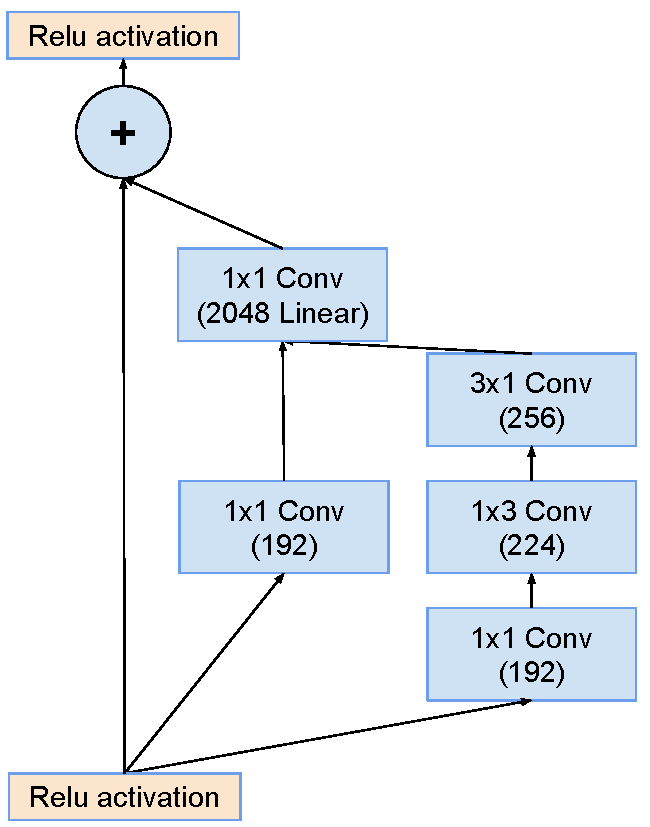
\includegraphics[width=\linewidth]{resnetwide8x8}
\caption{The schema for $8\times 8$ grid  (Inception-ResNet-C) module of the
 Inception-ResNet-v2 network.}
\label{fig:resnetwide8x8module}
\end{figure}
\begin{table}
{\small
 \begin{center}
   \begin{tabular}[H]{|l|c|c|c|c|}
   \hline
   {\bf Network} & {$k$} & {$l$} & {$m$} & {$n$} \\
   \hline
   Inception-v4 & 192 & 224 & 256 & 384 \\
   Inception-ResNet-v1 & 192 & 192 & 256 & 384 \\
   Inception-ResNet-v2 & 256 & 256 & 384 & 384 \\
   \hline
   \end{tabular}
 \end{center}
 }
\caption{The number of filters of the Reduction-A module for the three
  Inception variants presented in this paper. The four numbers in the
  colums of the paper parametrize the four convolutions of Figure~\ref{fig:reductionto17} }
\label{reductionto17params}
\end{table}

\subsection{Scaling of the Residuals}
Also we found that if the number of filters exceeded 1000, the residual
variants started to exhibit instabilities and the network has just
``died'' early in the training, meaning that the last layer before the
average pooling started to produce only zeros after a few tens of thousands of
iterations. This could not be prevented, neither by lowering the learning
rate, nor by adding an extra batch-normalization to this layer.

We found that scaling down the residuals before adding them to
the previous layer activation seemed to stabilize the training. In general
we picked some scaling factors between 0.1 and 0.3 to scale the residuals
before their being added to the accumulated layer activations
(cf. Figure~\ref{fig:resnetscaling}).

A similar instability was observed by He et al. in~\cite{he2015deep} in
the case of very deep residual networks and they suggested a two-phase
training where the first ``warm-up'' phase is done with very low learning
rate, followed by a second phase with high learning rata. We found that
if the number of filters is very high, then even a very low (0.00001) learning
rate is not sufficient to cope with the instabilities and the training with
high learning rate had a chance to destroy its effects. We found it much
more reliable to just scale the residuals.

Even where the scaling was not strictly necessary, it never
seemed to harm the final accuracy, but it helped to stabilize the training.
\begin{figure}
\centering
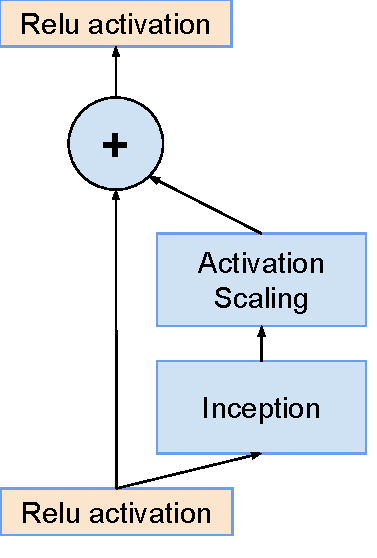
\includegraphics[width=0.4\linewidth]{resnetscaling}
\caption{The general schema for scaling combined Inception-resnet moduels.
  We expect that the same idea is useful in the general resnet case, where
instead of the Inception block an arbitrary subnetwork is used. The scaling
block just scales the last linear activations by a suitable constant, typically
around 0.1.}
\label{fig:resnetscaling}
\end{figure}
